\p
طبق شرایط مسئله صفحه را به دلخواه، به موزاییک‌های 
$3\times1$ 
تقسیم می‌کنیم. بدیهی است که یک خانه اضافه می‌آید.
	\p
\begin{center}
    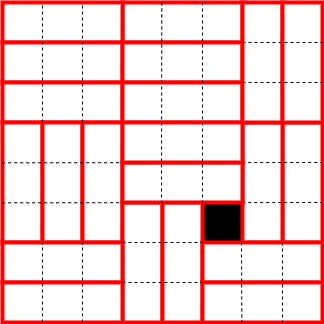
\includegraphics[height=3.5cm]{0.png}
\end{center}
\vspace*{+0.5cm}
\begin{itemize}
	\item 
اگر خانه‌ی اضافی بنفش باشد، در
$21$ 
موزاییک ایجاد شده
$43$
خانه‌ی بنفش وجود دارد. طبق اصل لانه کبوتری حداقل 
$1$
موزاییک وجود دارد که هر 
$3$ 
خانه‌اش رنگ شده باشد:
$$\left \lceil \frac{43}{21} \right \rceil = 3$$ 
    \item 
اگر خانه‌ی اضافی بنفش نباشد، در
$21$ 
موزاییک ایجاد شده 
$44$
خانه‌ی بنفش وجود دارد. طبق اصل لانه کبوتری حداقل 
$1$
موزاییک وجود دارد که هر 
$3$ 
خانه‌اش رنگ شده باشد:
$$\left \lceil \frac{44}{21} \right \rceil = 3$$ 
\end{itemize}
\p
در نتیجه
با توجه به شکل در نظر گرفته شده برای موزاییک‌ها، 	  
$3$
 خانه متوالی در یک سطر یا ستون وجود دارند که هر سه به رنگ بنفش باشند.
